%!TEX root = ../mieic.tex

\chapter{Projeto}
\label{chap:chap3}

\section*{}

O principal objetivo desta dissertação, como foi referido no capítulo \ref{chap:intro}, é desenvolver um (ou mais) módulo(s) de software que contribuam para uma melhoria na descoberta e recomendação de música num ambiente integrado entre o RAMA e o Spotify, por forma a tirar partido da representação gráfica do grafo de artistas de música do RAMA e da qualidade do serviço de \emph{Streaming} de música do Spotify.

Para tal, a proposta inicial desta dissertação consiste em desenvolver, no mínimo, um módulo que implemente uma das seguintes funcionalidades:

\begin{enumerate}
  \item \label{item:obj1} Integrar o serviço de \emph{streaming} de música do Spotify \textbf{no RAMA}
  \item \label{item:obj2} Integrar informação de um utilizador Spotify \textbf{no RAMA}
  \item \label{item:obj3} Melhorar design e funcionalidades \textbf{do RAMA}
  \item \label{item:obj4} Integrar a visualização de grafos de artistas de música \textbf{numa Aplicação Spotify}
  \item \label{item:obj5} Integrar o módulo de criação de \emph{playlists} do RAMA \textbf{numa Aplicação Spotify}
  \item \label{item:obj6} Integrar alguns dos módulos acima referidos \textbf{numa aplicação móvel}
\end{enumerate}

As três primeiras funcionalidades (\ref{item:obj1}, \ref{item:obj2} e \ref{item:obj3}) focam-se em melhorar o serviço do RAMA, usando API's do Spotify, ou seja, integrar o Spotify dentro do RAMA.
Por outro lado, as funcionalidades \ref{item:obj4} e \ref{item:obj5} têm como objetivo integrar o RAMA dentro do Spotify, através de uma Aplicação Spotify, que funciona como \emph{plugin} do programa principal do Spotify.
A última funcionalidade (\ref{item:obj6}) teria de implementar algumas das anteriores num Sistema Operativo Móvel (Android, iOS ou Windows Phone).

Este capítulo procura analisar todas as condicionantes que afetam a escolha  dos módulos a desenvolver, e em que ambientes estes se encaixam melhor (Aplicação Spotify, aplicação móvel ou RAMA).

Inicialmente será explorado o ambiente de desenvolvimento que o Spotify disponibiliza, ou seja, que tecnologias tem disponíveis para \emph{developers}.
De seguida serão analisadas quais dessas tecnologias assentam melhor em cada um dos módulos propostos a desenvolver, através de experimentações feitas, e quando necessário, será descrito um possível esquema de arquitetura por forma a facilitar a explicação do problema.


No final deste capítulo, deve ficar claro quais serão os módulos de software a desenvolver, que tecnologias irão ser usadas e qual o esquema geral da sua arquitetura.
O produto final deve de ir ao encontro do objetivo de contribuir para uma melhoria na descoberta e recomendação de música num ambiente relacionado com o RAMA.


\section{Spotify} % (fold)
\label{sec:spotify}

  O Spotify é um serviço de \emph{streaming} de música que permite ouvir, através de uma ligação de Internet, qualquer música que o Spotify possua no seu catálogo.


  \subsection{Ferramentas de Desenvolvimento} % (fold)
  \label{sub:ferramentas_de_desenvolvimento}
  
    No momento de escrita deste relatório, o Spotify tem disponível um conjunto de ferramentas\footnote{http://developer.spotify.com/technologies} para desenvolver módulos de software que podem estar embebidos nas mais diversas aplicações (\emph{third-party applications}) ou então dentro do \emph{Spotify Desktop Client}.

    Existem quatro ferramentas de desenvolvimento, cada uma delas com o seu propósito e utilidade.


    \subsubsection{Spotify Apps} % (fold)
    \label{ssub:spotify_apps}
      Serve para desenvolver Aplicações Spotify\footnote{https://developer.spotify.com/technologies/apps} que são usadas pelos utilizadores Spotify dentro do \emph{Spotify Desktop Client}. Estas são aplicação \emph{HTML5}\footnote{http://www.w3.org/TR/html5/}.

      \begin{figure}
        \begin{center}
          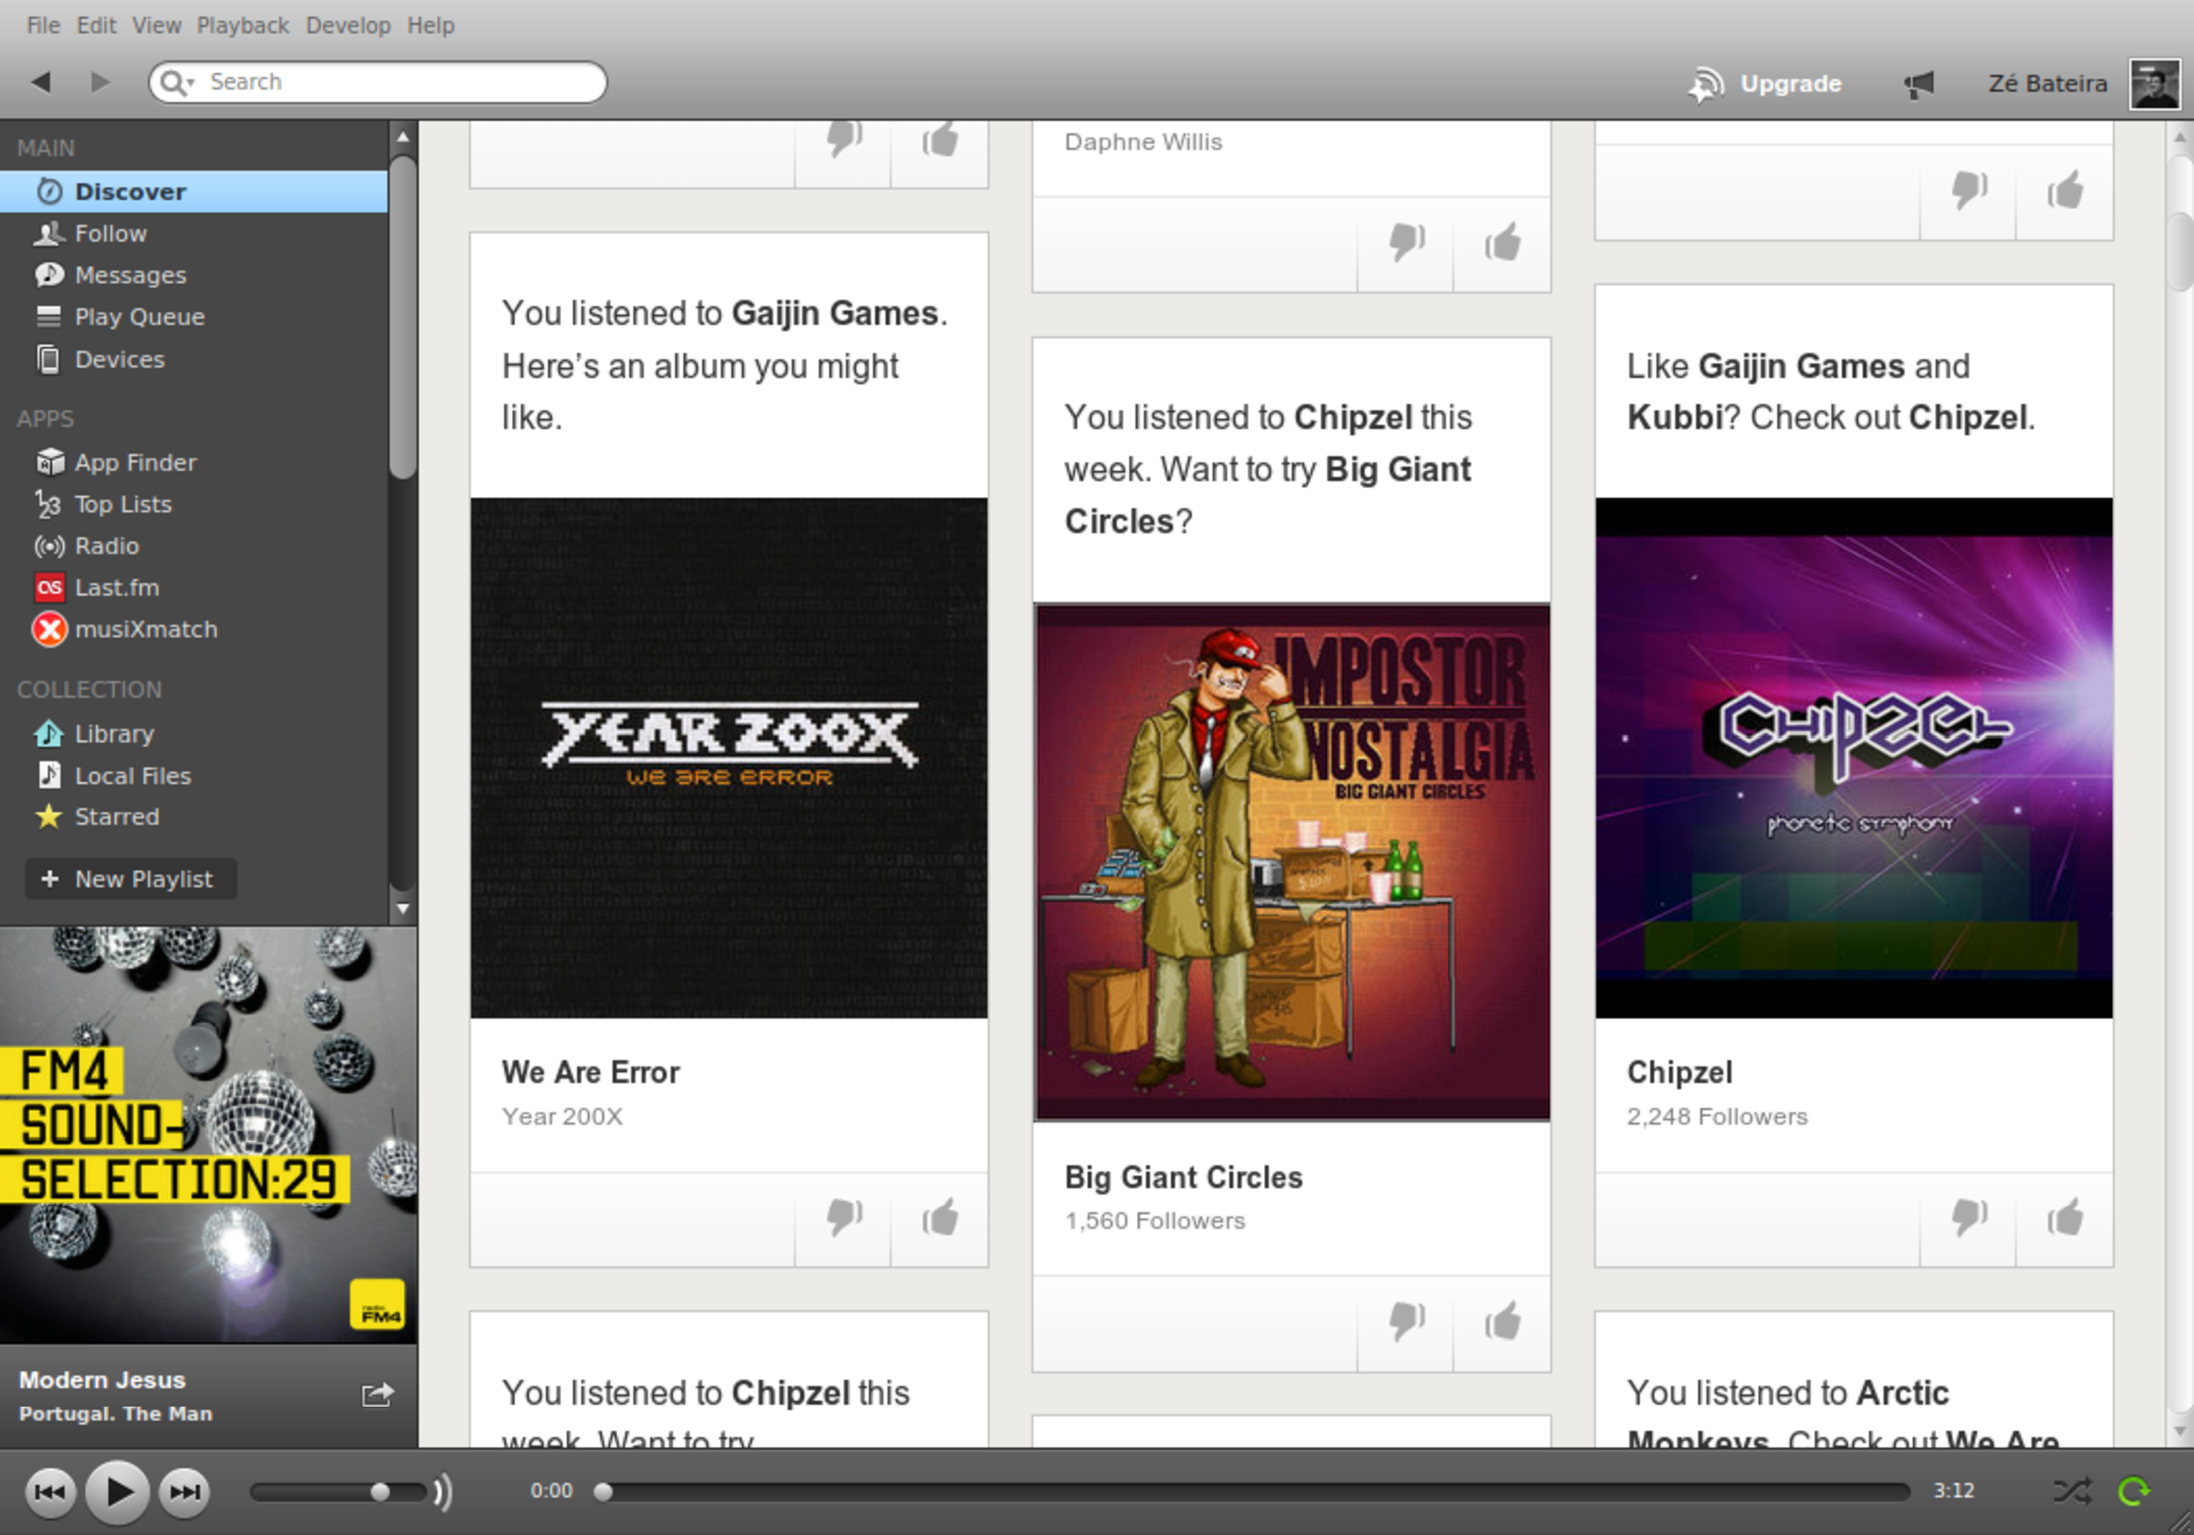
\includegraphics[width=\textwidth]{spotify.pdf}
        \end{center}
        \caption{Spotify: interface do modo de descoberta do \emph{desktop client}}
        \label{fig:spotify_apps}
      \end{figure}

      Na figura \ref{fig:spotify_apps} é possível ver o aspeto do \emph{Spotify Desktop Client}.
      Na barra lateral esquerda, dentro do separador \emph{Apps}, aparece a lista de aplicações já instaladas, assim como o \emph{App Finder}, que permite procurar e instalar aplicações com apenas um clique.
 
      Na figura \ref{fig:spotify_apps2} está aberta a aplicação da Last.fm. É possível ver que as Aplicações Spotify têm apenas um espaço reservado embutido no \emph{Spotify Desktop Client}.

      \begin{figure}
        \begin{center}
          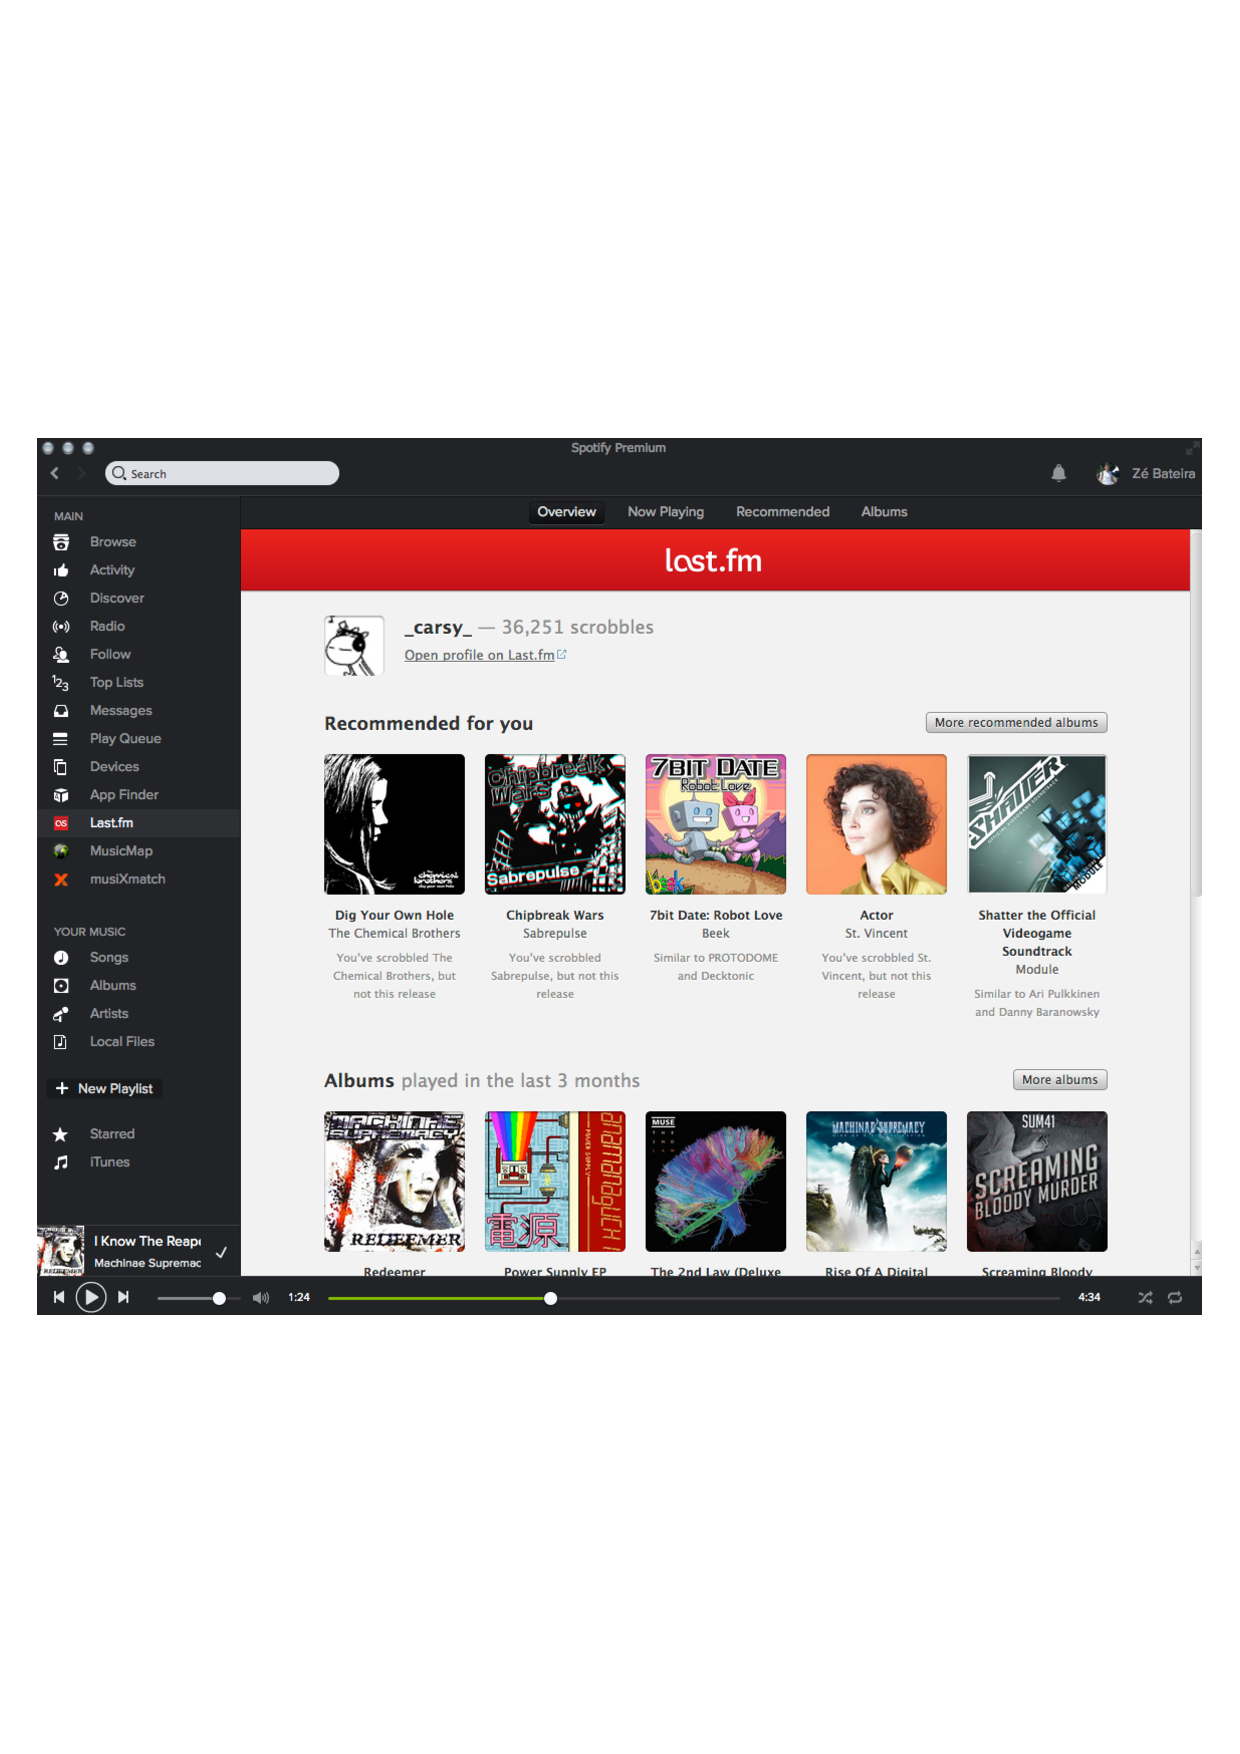
\includegraphics[width=\textwidth]{spotify_apps.pdf}
        \end{center}
        \caption{Spotify: Aplicação Last.fm aberta no \emph{Spotify Player}}
        \label{fig:spotify_apps2}
      \end{figure}

      Para o seu desenvolvimento destas aplicações são disponibilizadas duas \emph{frameworks}: \emph{API Framework}\footnote{https://developer.spotify.com/docs/apps/api/1.0/} e \emph{Views Framework}\footnote{https://developer.spotify.com/docs/apps/views/1.0/}.
      A primeira fornece uma interface para recolher metadados de artistas, álbuns e músicas e controlar o reprodutor de música.
      A segunda fornece componentes de design como botões, listas, abas, entre outros, para o desenvolvimento da aplicação.

      Para desenvolver os módulos \ref{item:obj4} e \ref{item:obj5} esta é a ferramenta mais apropriada.

    % subsubsection spotify_apps (end)


    \subsubsection{Spotify Widgets} % (fold)
    \label{ssub:spotify_widgets}
      As Widgets\footnote{https://developer.spotify.com/technologies/widgets} são pequenos componentes que se podem embeber em \emph{websites}.
      No momento da escrita deste relatório existem dois componentes: \emph{Play Button} (\ref{fig:spotify_play_button}) e \emph{Follow Button} (\ref{fig:spotify_follow_button}).

      \begin{figure}
        \begin{center}
          
\includegraphics{spotify_play_button.pdf}
        \end{center}
        \caption{Spotify: \emph{Play Button} pode ser embebido em \emph{websites}.}
        \label{fig:spotify_play_button}
      \end{figure}

      \begin{figure}
        \begin{center}
          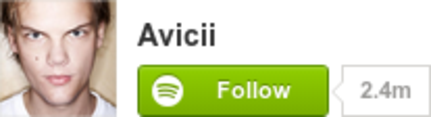
\includegraphics{spotify_follow_button.pdf}
        \end{center}
        \caption{Spotify: \emph{Follow Button} permite seguir um artista.}
        \label{fig:spotify_follow_button}
      \end{figure}

      No entanto, existe algumas limitações no uso destas componentes.
      No Spotify, apenas utilizadores que tenham criado conta no serviço Spotify é que podem usar o mesmo.
      O mesmo também se aplica a estas \emph{widgets} - apesar de estas existirem numa aplicação externa ao Spotify, apenas utilizadores Spotify podem usá-las.
      Esta limitação pode fazer sentido para o \emph{Follow Button}, mas o \emph{Play Button} torna-se inútil para utilizadores que não usem o Spotify.
      Outro problema surge quando a música do \emph{Play Button} não está disponível no País em que o utilizador está.

      Estas \emph{widgets} apenas servem de hiperligação ou ao \emph{Player} do Spotify ou ao \emph{WebPlayer} do Spotify.
      Na realidade, usando estas \emph{widgets}, o stream de música do Spotify é sempre reproduzido dentro do ambiente do Spotify, e nunca em aplicações externas. \\

      Para embeber as \emph{widgets} apenas é necessário introduzir um elemento \emph{iframe} no código \emph{HTML} fonte do \emph{website}:

      \lstinputlisting[language=HTML,caption={Código \emph{HTML} para embeber um \emph{Play Button}}]{snippets/play_button.html}

      As \emph{widgets} seriam úteis para desenvolver os módulos \ref{item:obj1} e \ref{item:obj3}.

    % subsubsection spotify_widgets (end)

    \subsubsection{Libspotify SDK} % (fold)
    \label{ssub:libspotify_sdk}
    
      Libspotify SDK\footnote{https://developer.spotify.com/technologies/libspotify} é uma API que permite adicionar os serviços do Spotify em aplicações externas.
      No entanto, existem algumas limitações para os utilizadores destas aplicações.
      
      Existem, dois tipos de conta a que o utilizador pode subscrever: conta grátis e conta \emph{premium}.
      Como foi referido anteriormente (\ref{ssub:spotify_widgets}) apenas utilizadores Spotify podem interagir com qualquer componente do Spotify, dentro ou fora das aplicações nativas do mesmo.
      Libspotify fornece uma interface que permite a um utilizador fazer \emph{login} no Spotify em aplicações externas por forma a poder ouvir música do Spotify, criar playlists e outras funcionalidades.
      No entanto, os únicos utilizadores que pode fazer \emph{login} nestas aplicações que usam Libspotify, são utilizadores \emph{premium}.
      Para além de que, os \emph{developers} da própria aplicação também precisam de ser utilizadores \emph{premium}.

      Neste sentido, uma aplicação que, para funcionar, necessita de que o utilizador, para além de possuir uma conta Spotify, também pague uma subscrição mensal \emph{premium}, é uma aplicação bastante restritiva.

      Esta ferramenta pode ser usada para desenvolver os módulos \ref{item:obj1}, \ref{item:obj2} e \ref{item:obj6}.
      

    % subsubsection libspotify_sdk (end)


    \subsubsection{Metadata API} % (fold)
    \label{ssub:metadata_api}
    
      A \emph{Metadata API}\footnote{https://developer.spotify.com/technologies/web-api} disponibiliza publicamente informação de músicas, álbuns e artistas da Base de dados do Spotify.

      Através de pedidos HTTP é possível obter informação da base de dados do Spotify. Existe dois tipos de pedidos que esta API disponibiliza: \emph{search}\footnote{https://developer.spotify.com/technologies/web-api/search} e \emph{lookup}\footnote{https://developer.spotify.com/technologies/web-api/lookup}.
      Para obter informação detalhada de, por exemplo, um artista, é necessário saber o deu identificador único.
      Esse identificador é um \emph{URI} da forma:

      \url{spotify:artist:<artist_id>}, onde \emph{artist\_id} é um identificar único.

      Exemplo:

      \url{spotify:artist:65nZq8l5VZRG4X445F5kmN}, é o identificador único da fadista "Mariza". \\

      Também existem identificadores únicos para álbuns:

      \url{spotify:album:5d1LpIPmTTrvPltx26TlEU} (álbum "Fado Tradicional" de "Mariza") \\

       e para faixas de música:

       \url{spotify:track:2vqYasauhDLVjTt7CGWK6y} (música "Fado Vianinha" do mesmo álbum) \\

      Para obter este \emph{URI} é preciso interrogar a base de dados com um método de pesquisa.
      Para isso, usa-se o \emph{search}.

      \begin{description}
        \item[\emph{Search}] \hfill

          O \emph{URL} base de utilização é:

          \url{http://ws.spotify.com/search/1/album}, para pesquisa de álbuns.

          Se se pretender pesquisar Artistas, usa-se \emph{artist}, se se pretender pesquisar Faixas de música, usa-se \emph{track}. \\

          Exemplos:

          \url{http://ws.spotify.com/search/1/album?q=foo} \\
          \url{http://ws.spotify.com/search/1/artist.json?q=red+hot} \\

          O resultado da \emph{query}, por defeito, tem o formato \emph{XML}. No entanto, também se pode especificar o formato \emph{JSON} (como no segundo exemplo).

          Dada a \emph{query}: \\
          \url{http://ws.spotify.com/search/1/artist.json?q=camane} (fadista "Camané")

          Obtém-se o resultado:

          \lstinputlisting[caption={Os resultados são ordenados pelo atributo "popularity"}]{snippets/search_camane.json}

        \item[\emph{Lookup}] \hfill \\
          Depois de obtido o \emph{URI} identificador, é possível obter mais informações de um conteúdo usando o \emph{lookup}.

          A seguinte \emph{query}: \\
          \url{http://ws.spotify.com/lookup/1/.json?uri=spotify:artist:3MLPFTe4BrpEV2eOVG0gLK}

          Retorna:

          \lstinputlisting[caption={Resultado do \emph{lookup} do fadista "Camané"}]{snippets/lookup_camane.json}

      \end{description}

      Esta API seria bastante útil para desenvolver qualquer um dos seis módulos propostos.
      Aliás, até complementa as \emph{Widgets} e o \emph{Libspotify SDK}.

    % subsubsection metadata_api (end)

  % subsection ferramentas_de_desenvolvimento (end)

  \subsection{Experimentações Feitas} % (fold)
  \label{sub:experimentacoes}
  
    Numa primeira experiência com as ferramentas, foi criado um pequeno \emph{website} que permite pesquisar e ouvir Música do Spotify usando a \emph{Metadata API} e \emph{Spotify Widgets}: \\

    \url{http://carsy.github.io/spotify-playground} \\

    Na figura \ref{fig:playground} é possível ver o resultado de uma pesquisa, e a \emph{Widget Play Button} com o resultado selecionado da pesquisa.

    \begin{figure}
      \centering

      \begin{subfigure}[b]{0.38\textwidth}
        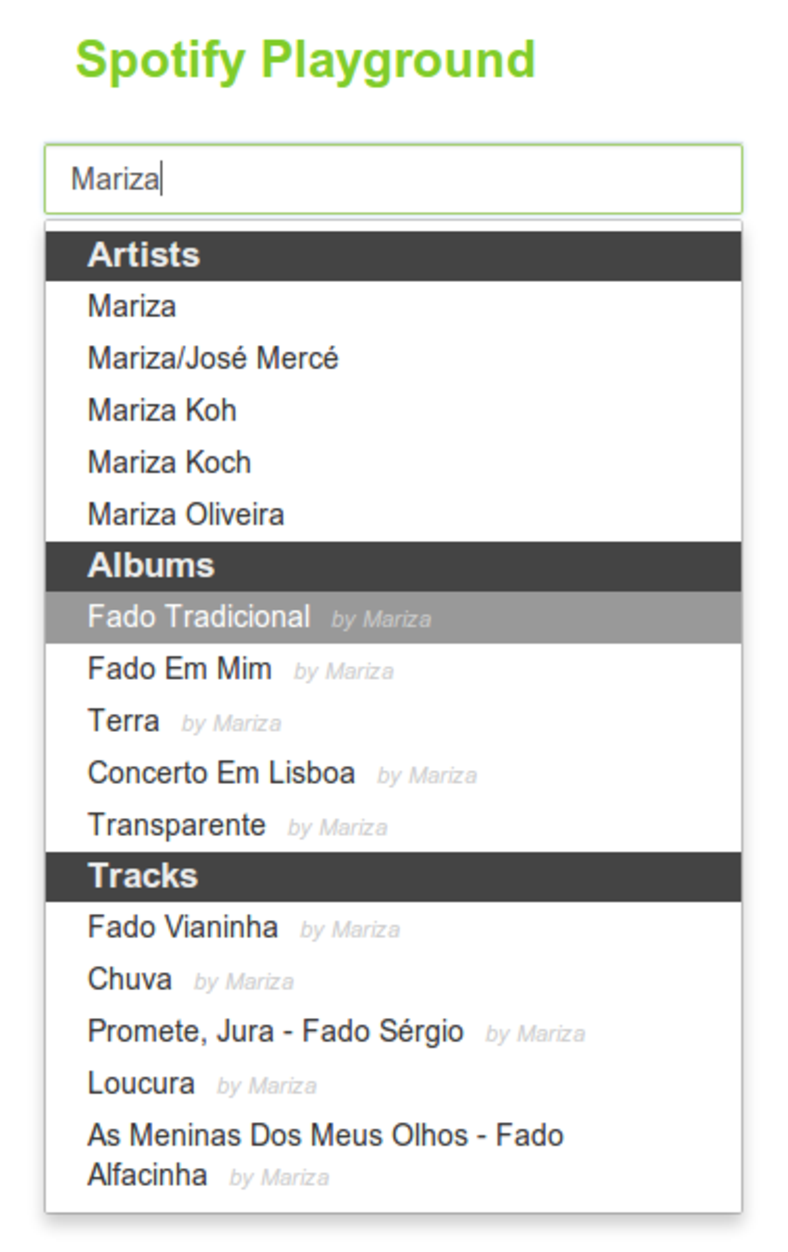
\includegraphics[width=\textwidth]{playground.pdf}
        \caption{Resultado da pesquisa "Mariza"}
        \label{fig:playgroun_a}
      \end{subfigure}

      \begin{subfigure}[b]{0.38\textwidth}
        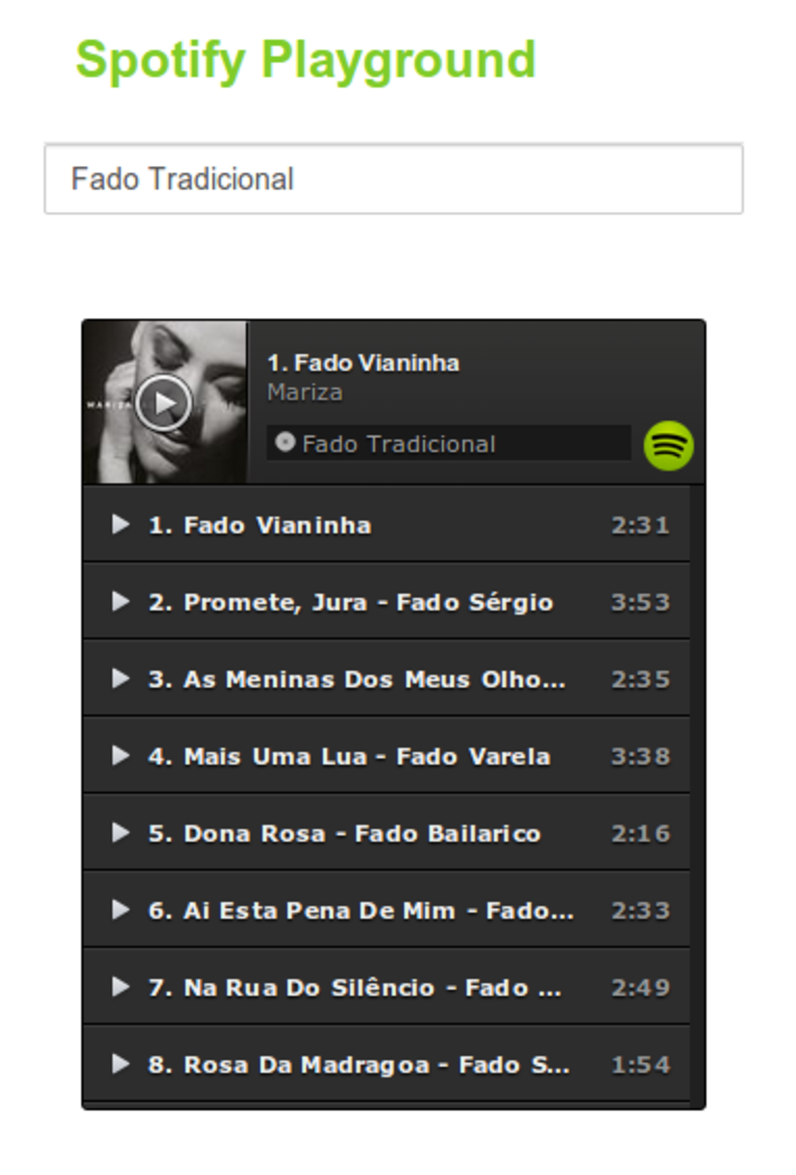
\includegraphics[width=\textwidth]{playground2.pdf}
        \caption{Depois de selecionado o álbum "Fado Tradicional" aparece o \emph{Play button} com as faixas do álbum.}
        \label{fig:playground_b}
      \end{subfigure}

      \caption{Experiência com \emph{Metadata API} e \emph{Play Button Widget} (código fonte: \url{github.com/carsy/spotify-playground})}
      \label{fig:playground}

    \end{figure}

    Verificou-se que as duas ferramentas estão bem documentadas e em constante atualização. \\

    Outra experiência foi realizada para verificar se é possível usar o elemento \emph{canvas} numa Aplicação Spotify.
    Isto é necessário pois será a única forma de poder desenhar graficamente o grafo.
    Para isso foi apenas necessário criar uma aplicação com o seguinte código fonte:

    \begin{lstlisting}[caption={Elemento \emph{iframe} que embebe o \emph{website} do RAMA na aplicação}]
      <iframe src="http://rama.inescporto.pt/app" frameborder="0"></iframe>\end{lstlisting}

    Desta forma, é possível embeber o RAMA na Aplicação Spotify (que usa o elemento \emph{canvas} para desenhar o grafo).
    Resultado final na figura \ref{fig:rama_spotifyed}.

    \begin{figure}
      \begin{center}
        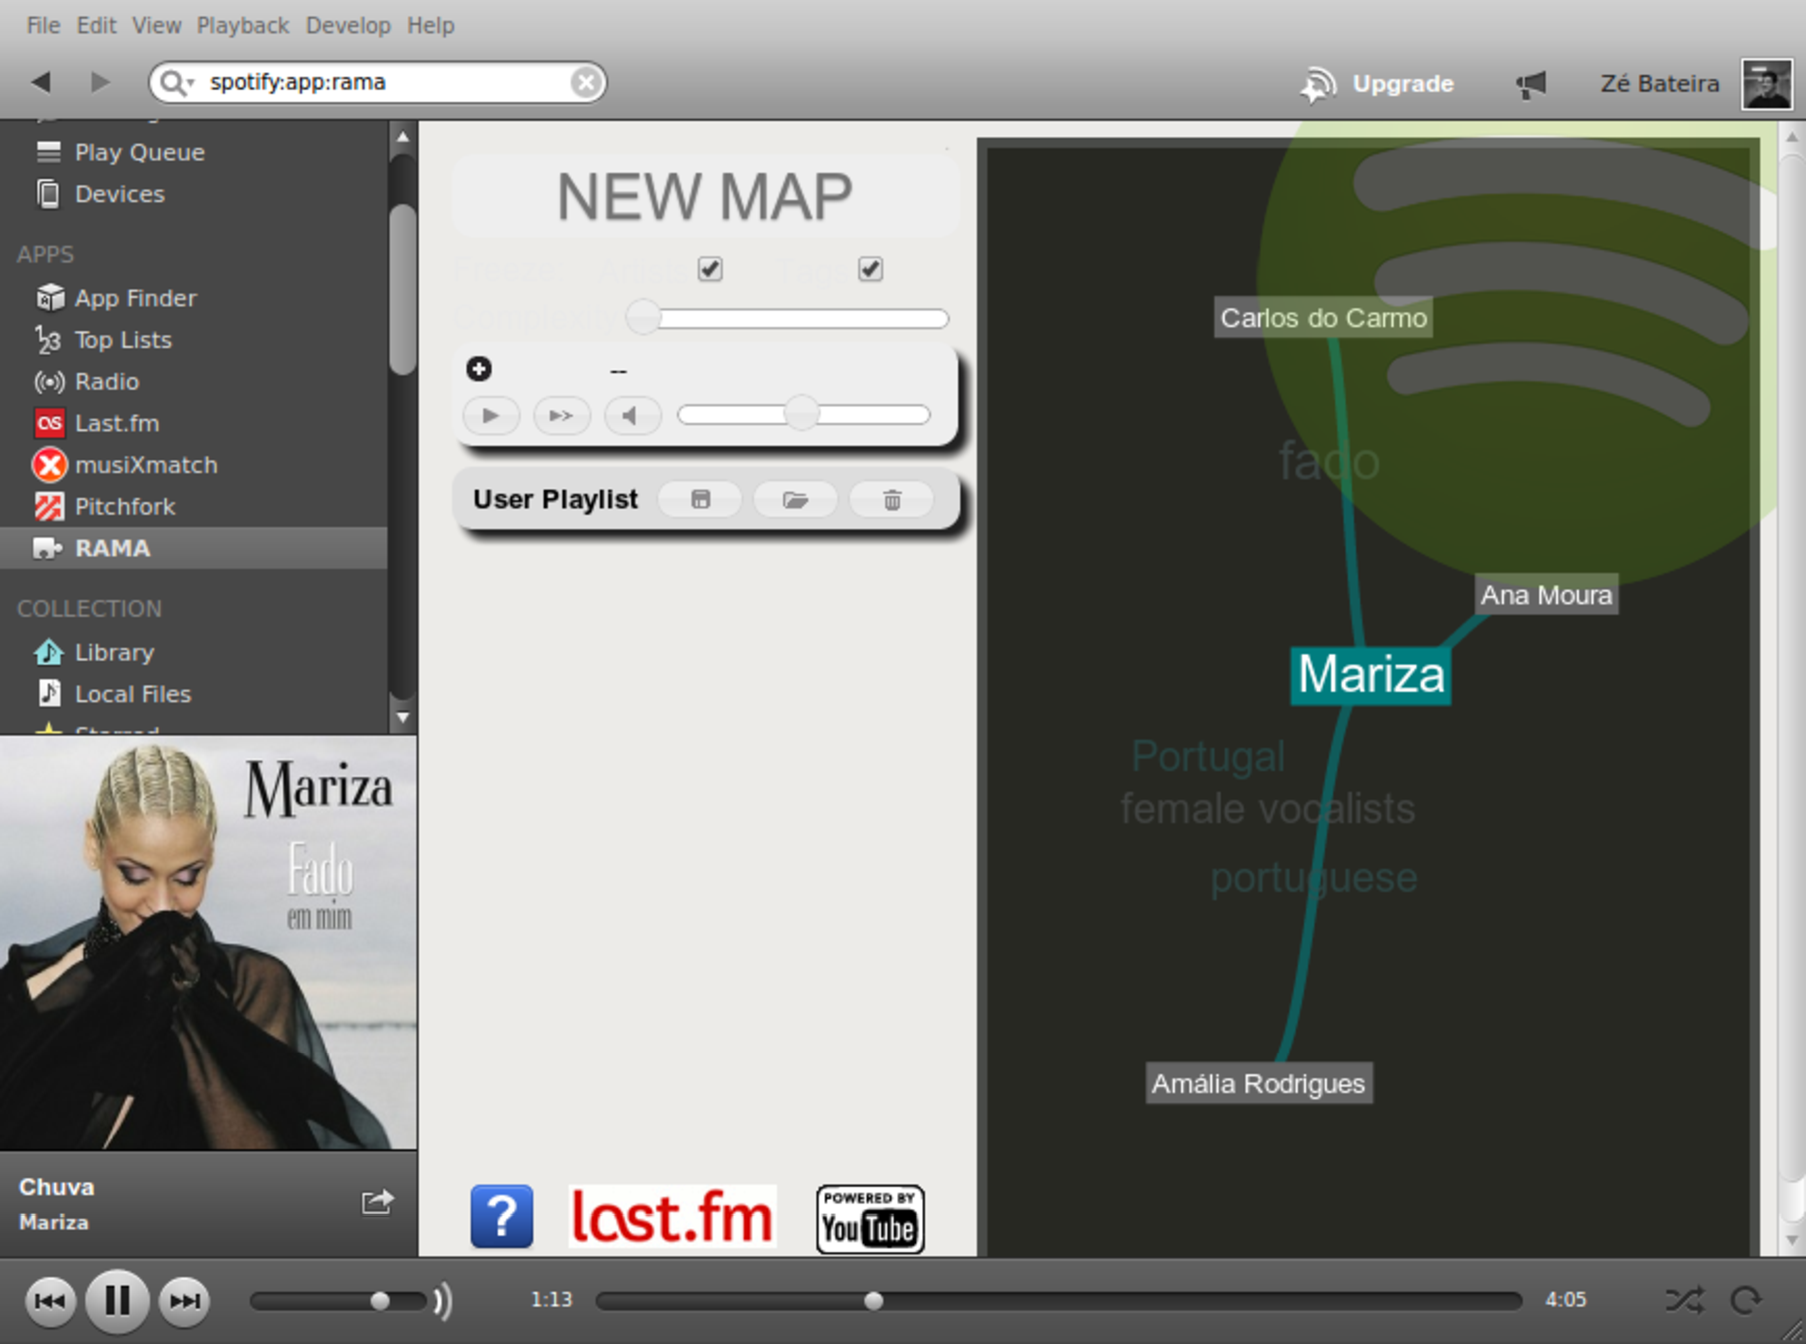
\includegraphics[width=\textwidth]{rama.pdf}
      \end{center}
      \caption{\emph{Website} do RAMA embebido numa Aplicação Spotify}
      \label{fig:rama_spotifyed}
    \end{figure}

    Apesar de \emph{iframes} serem suportadas, existem outros componentes que não o são.
    A aplicação não é usável, pois não permite, por exemplo, reproduzir automaticamente faixas de artistas.

    No entanto existe uma forma de testar quais os elementos de \emph{HTML5} suportados, usando uma aplicação interna do Spotify.
    Na figura \ref{fig:canvas_support} é possível ver que o elemento \emph{canvas} é suportado a cem por cento.

    \begin{figure}
       \begin{center}
         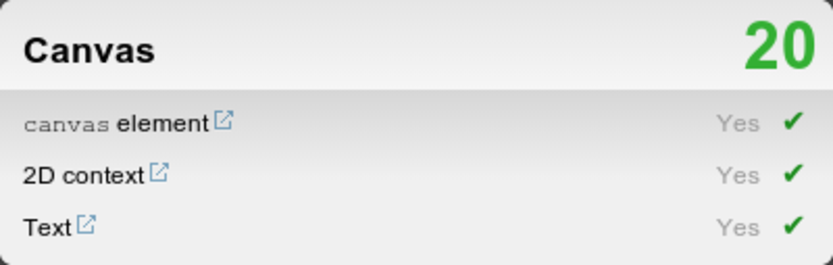
\includegraphics[width=0.5\textwidth]{canvas_support.pdf}
       \end{center}
       \caption{Resultado do teste do elemento \emph{canvas}}
       \label{fig:canvas_support}
     \end{figure}

  % subsection experimentacoes (end)

  \subsection{Conclusão} % (fold)
  \label{sub:conclusao}
  
    A prova de conceito desenvolvida (\ref{fig:rama_spotifyed}) demonstrou-se a mais indicada para o objetivo final de criar um ambiente integrado entre o Spotify e o RAMA.

    Assim, os módulos a serem desenvolvidos são \ref{item:obj4} e \ref{item:obj5}.

  % subsection conclusao (end)

% section spotify (end)

\section{Tecnologias} % (fold)
\label{sec:tecnologias}

  As seguintes tecnologias serão utilizadas nas fase de desenvolvimento, testes e otimização da Aplicação Spotify.

  \subsection{\emph{Spotify Desktop Client}} % (fold)
  \label{sub:subsection_name}
    O desenvolvimento de Aplicações Spotify é feito de forma integrada no programa.

    Para abrir uma Aplicação Spotify, localmente, escreve-se o seguinte na barra de pesquisa: spotify:app:rama

    Onde \emph{rama} deve ser o identificador da aplicação declarado no ficheiro \emph{manifest.json}\footnote{ficheiro situado na \emph{root} da pasta do projeto}. \\
    Exemplo de ficheiro \emph{manifest.json}:

    \lstinputlisting[caption={manifest.json: \emph{BundleIdentifier} é o identificador da aplicação; \emph{Dependencies} declara as dependências das API's necessárias ao desenvolvimento.}]{snippets/manifest.json}

    Existem outras opções úteis a que se pode aceder usando a tab \emph{Develop} (\ref{fig:html5_support}).
    A opção "Show Inspector" abre a janela \emph{Webkit Development Tools} (\ref{sub:webkit_tools})

    \begin{figure}
      \begin{center}
        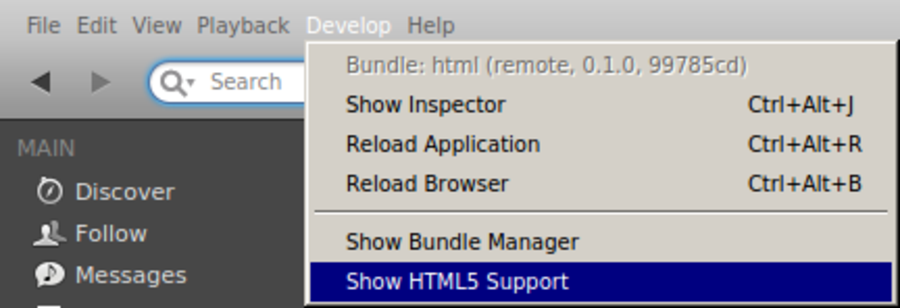
\includegraphics[width=0.6\textwidth]{html5_support.pdf}
      \end{center}
      \caption{Menu \emph{Develop}}
      \label{fig:html5_support}
    \end{figure}
  
  % subsection subsection_name (end)

  \subsection{Webkit Development Tools - webkit.org} % (fold)
  \label{sub:webkit_tools}

    A partir do \emph{webkit}, tem-se acesso a várias ferramentas úteis para o desenvolvimento \emph{web} (\ref{fig:webkit_inspector}).

    \begin{figure}
      \begin{center}
        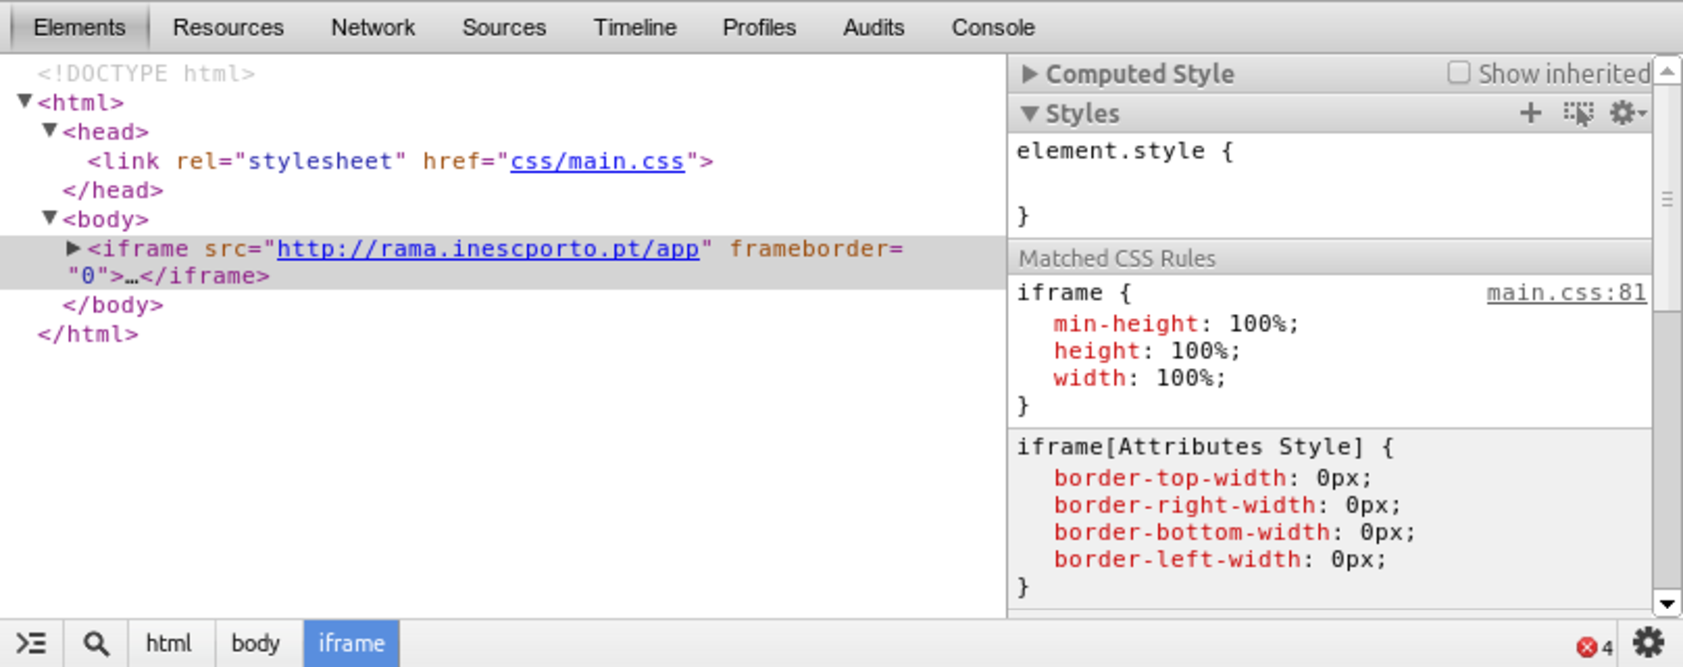
\includegraphics[width=\textwidth]{webkit_inspector.pdf}
      \end{center}
      \caption{Webkit: Vista da tab \emph{Inspector}. Outas ferramentas disponíveis (tabs): \emph{Resources, Network, Sources, Timeline, Profiles, Audits} e \emph{Console}.}

      \label{fig:webkit_inspector}
    \end{figure}

    A mais importantes são:

    \begin{description}
      \item[Inspector] Permite inspecionar e editar o código \emph{HTML} e \emph{CSS} da aplicação diretamente  (\ref{fig:webkit_inspector}).
      \item[Network] Permite, por exemplo, ver o tempo que cada componente da aplicação demorou a carregar (uma imagem ou um ficheiro \emph{css}) (\ref{fig:webkit_network}).
      \item[Profile] Permite identificar que partes do código \emph{javascript} são as mais frequentemente executadas (\ref{fig:webkit_profile}).
      \item[Audit] Ajuda a perceber quantos recursos estão a ser descarregados desnecessariamente, como por exemplo, regras de \emph{CSS} que não estão a ser usadas (\ref{fig:webkit_audit}).
      \item[Console] Muito útil para \emph{debug} de \emph{javascript}.

    \end{description}


    \begin{figure}
      \begin{center}
        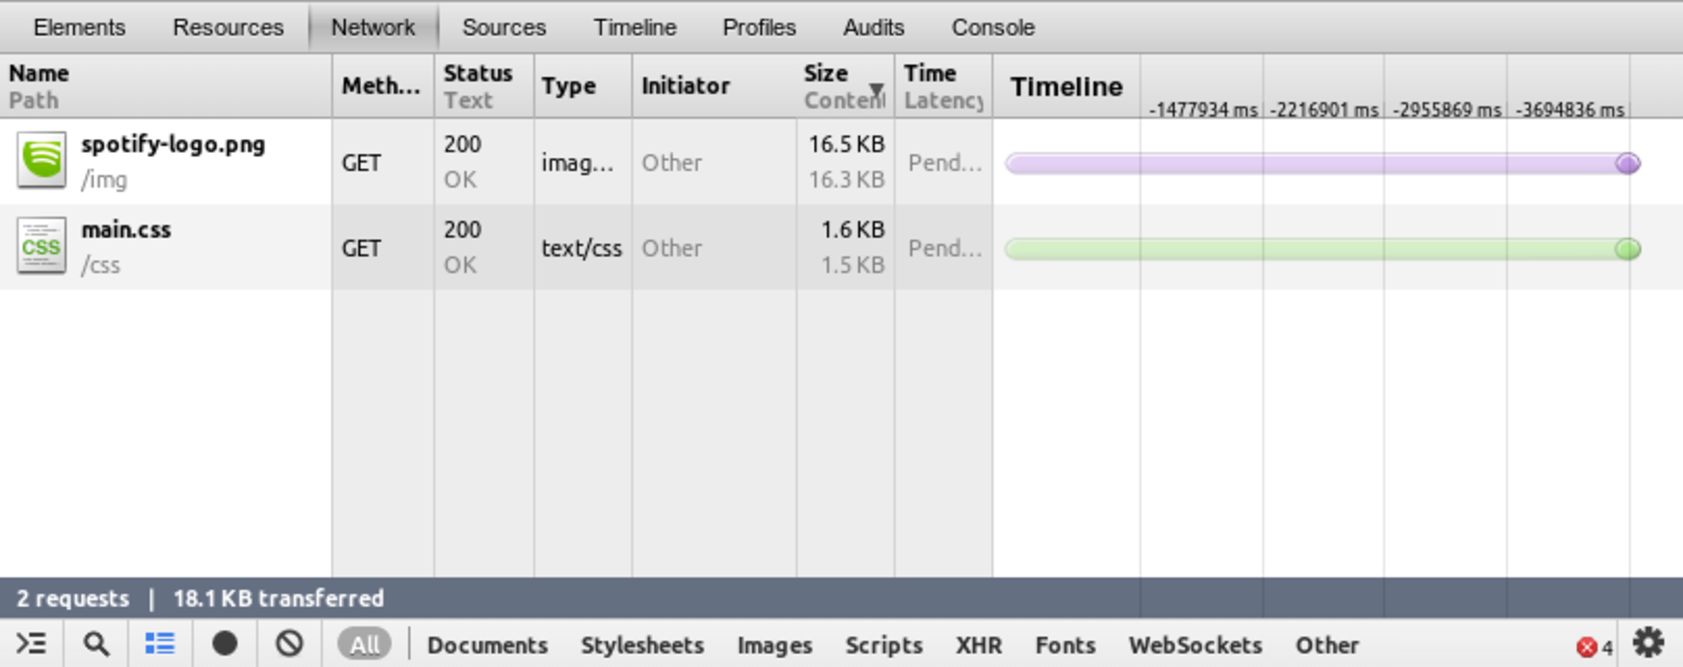
\includegraphics[width=\textwidth]{webkit_network.pdf}
      \end{center}
      \caption{Webkit Network}
      \label{fig:webkit_network}
    \end{figure}

    \begin{figure}
      \begin{center}
        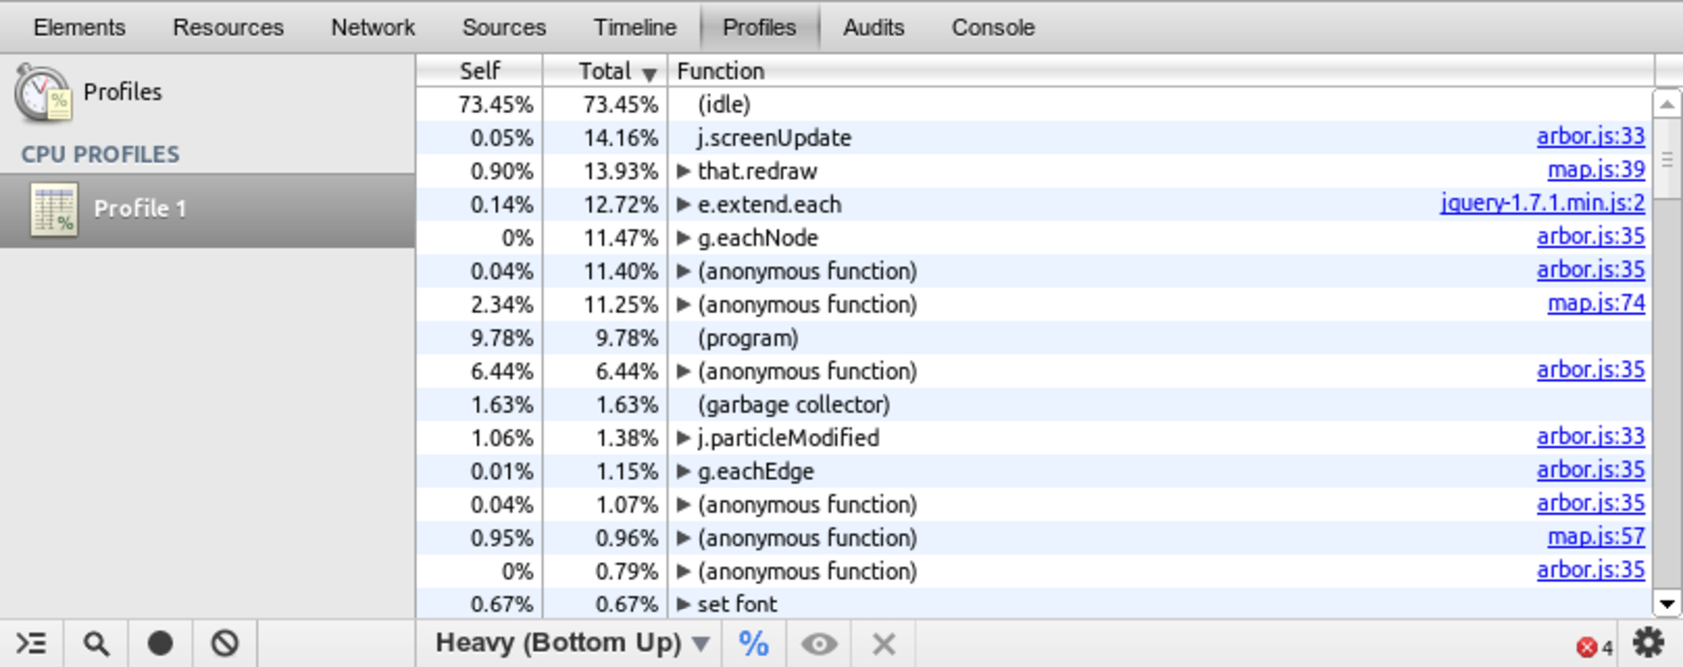
\includegraphics[width=\textwidth]{webkit_profile.pdf}
      \end{center}
      \caption{Webkit Profile: É possível ver que a renderização do grafo é o que ocupa mais tempo de processamento como esperado. No entanto, existe uma parte de \emph{JQuery} que ocupa 12.72\% do tempo de processamento, o que pode indicar um possível ponto de melhoria de performance.}
      \label{fig:webkit_profile}
    \end{figure}

    \begin{figure}
      \begin{center}
        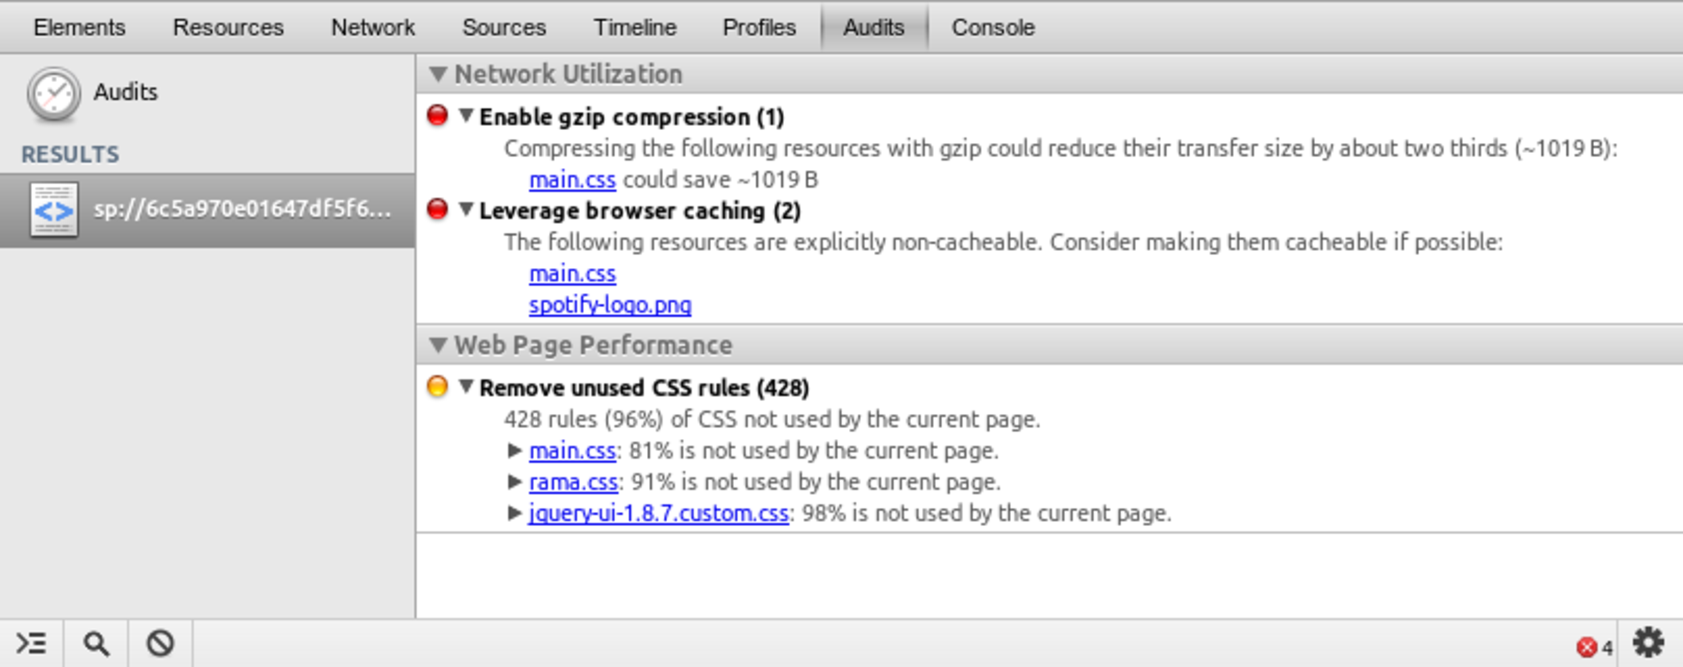
\includegraphics[width=\textwidth]{webkit_audit.pdf}
      \end{center}
      \caption{Webkit Audit: 96\% do código \emph{CSS} não está a ser usado, sendo por isso, um ponto de melhoria reduzir a quantidade de informação descarregada.}
      \label{fig:webkit_audit}
    \end{figure}

    \begin{figure}
      \begin{center}
        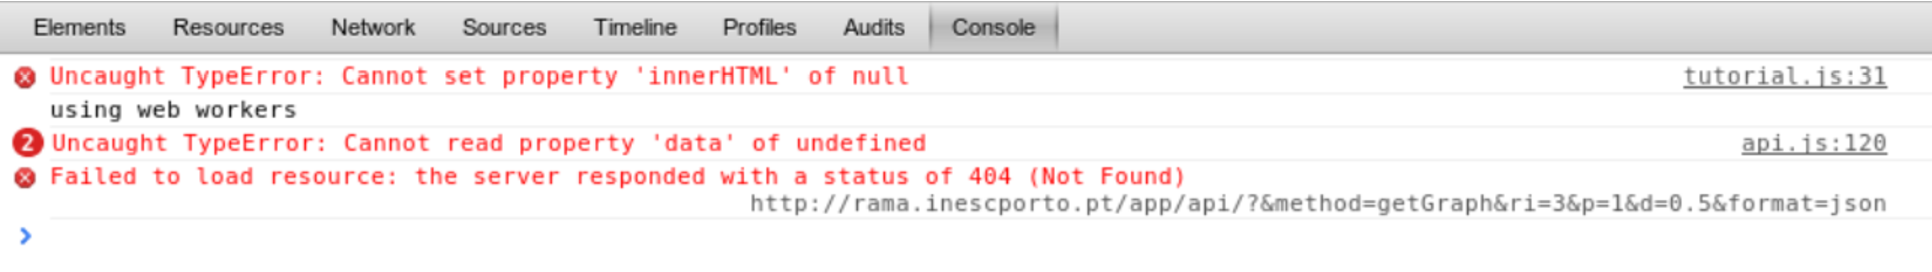
\includegraphics[width=\textwidth]{webkit_console.pdf}
      \end{center}
      \caption{Webkit Console: Erros de \emph{Javascript} aparecem destacados para chamar a atenção.}
      \label{fig:webkit_console}
    \end{figure}

  % subsection webkit_tools (end)

  \subsection{Npmjs - npmjs.org} % (fold)
  \label{sub:npm}
    Gestor de pacotes de software e dependências.
    Para usar \emph{npm} é necessário um ficheiro de configuração \emph{package.json} que permite identificar quais os pacotes de que a aplicação depende, e as suas versões. \\
    Exemplo:

    \lstinputlisting[caption={\emph{package.json}: ao indicar a versão com "*", significa que se deve usar sempre a mais recente.}]{snippets/package.json}

  % subsection npm (end)

  \subsection{Gruntjs - gruntjs.com} % (fold)
    \label{sub:gruntjs} 
      Programa de gestão de tarefas automatizadas.
      Muito útil para testes, compilação e otimização de código.
      É possível por exemplo, quando qualquer parte do código mudar, a aplicação automaticamente atualiza com as mudanças mais recentes, sem ser preciso refrescar manualmente a aplicação.
  % subsection gruntjs (end)

  \subsection{Arborjs - arborjs.org} % (fold)
  \label{sub:arborjs}
    Framework de javascript para desenho de grafos. Foi já utilizada no desenvolvimento do RAMA (existe sempre a possibilidade de se usar outra ferramenta substituta caso esta não for adequada).
  
  % subsection arborjs (end)

% section tecnologias (end)

\section{Resumo e Conclusões}

  A escolha final do módulo a desenvolver é a Aplicação Spotify.

  Apesar de as outras opções serem também viáveis, a possibilidade de poder integrar uma interface estilo RAMA num ambiente que os utilizadores já se sentem confortáveis (Spotify), é muito favorável a que seja melhor aceite pelos mesmos.

  É esperado que as tecnologias a usar ajudem no desenvolvimento desta dissertação.

  Em suma, será desenvolvida uma Aplicação Spotify que implemente os módulos \ref{item:obj4} e \ref{item:obj5}.